\documentclass[10pt,a4paper,twocolumn]{article}
\usepackage[utf8]{inputenc}
\usepackage[T1]{fontenc}
\usepackage[spanish]{babel}
\usepackage{lmodern,graphicx,csquotes}
\usepackage[margin=1.65cm,columnsep=.65cm]{geometry}

\usepackage[backend=biber,style=ieee,url=false,isbn=false,maxbibnames=3]{biblatex}
\usepackage[colorlinks=true,allcolors=teal]{hyperref}
\usepackage{xcolor}
\addbibresource{../referencias/referencias-kevin.bib}
\addbibresource{../referencias/referencias-joseph.bib}
\addbibresource{../referencias/referencias-juliana.bib}
\addbibresource{../referencias/referencias-complementarias.bib}
\IfFileExists{../referencias/referencias-khriz.bib}{\addbibresource{../referencias/referencias-khriz.bib}}{}
\setlength{\parindent}{0pt}
\setlength{\parskip}{3pt}
\emergencystretch=2em
\DefineBibliographyStrings{spanish}{artno={art.}}
\begin{document}
\twocolumn[{
\centering
{\LARGE\bfseries Servicios web: SOAP y REST\par}
\smallskip
{\large Aplicación a la evolución de nuestros PFC\par}
\smallskip
{\small Aplicaciones Distribuidas · GA-SUM-01 / EXP-1 · Grupo CCEG\par}
\medskip
}]
\section{Kevin García: consulta REST en el RTV}



\subsection{Sistema y operación}

El sistema de Revisión Técnica Vehicular gestiona turnos, pagos e inspecciones. El personal utiliza una aplicación web conectada al backend. La operación analizada es la consulta del estado de un turno desde una aplicación para solicitantes.



\subsection{Arquitectura propuesta}

Se propone incorporar un servicio REST de consulta con una base de lectura independiente. El backend conservaría la base principal de turnos y pagos, y los cambios confirmados se propagarían mediante una cola de mensajes. Un consumidor actualizaría la base de lectura. La aplicación del solicitante consultaría el servicio REST mediante HTTP y recibiría una respuesta JSON.



Para publicar los cambios, el backend guardaría el turno y su evento en una misma transacción mediante una bandeja de salida. Un publicador enviaría los eventos registrados a la cola. El consumidor comprobaría el identificador y la versión del evento antes de actualizar la base de lectura, evitando procesar duplicados o reemplazar un estado reciente por otro anterior.



\subsection{Consulta REST}

La ruta propuesta es \texttt{GET /api/consulta/turnos/\{id\}}. El cliente envía el identificador del turno; no selecciona al propietario. El servicio verificaría la identidad del solicitante y su permiso para consultar el turno. Después leería la base de consulta y devolvería \texttt{200 OK} con un JSON que incluiría el identificador, el estado y la fecha de actualización. El número 123 del diagrama es ilustrativo. La demostración utiliza el turno 82.



El servicio devolvería un error controlado cuando el turno no exista o el usuario no tenga acceso, sin exponer información de terceros. La aplicación mostraría el estado recibido junto con su fecha de actualización.



\subsection{Qué oculta la distribución y qué debe informar}

En la propuesta, la aplicación del solicitante utiliza una dirección de consulta sin acceder directamente a las bases. Esto permite cambiar la ubicación interna de los datos sin cambiar la operación que usa el cliente. La respuesta JSON también evita que el cliente dependa de las tablas de PostgreSQL.



La distribución no se oculta por completo. Si la base de lectura todavía no recibe un cambio, la aplicación debe mostrar la fecha de actualización. Si la API no responde, debe informar el fallo. Ocultar esas situaciones podría hacer que el solicitante confunda un dato anterior con el estado vigente.



\subsection{Consistencia y manejo de fallos}

La propagación asíncrona permitiría atender consultas desde la base de lectura mientras se procesan los cambios de la base principal. Durante ese intervalo, el estado consultado podría corresponder a una versión anterior. La fecha de actualización permitiría identificar la antigüedad de la información.



Esta lectura se utilizaría para informar al solicitante. La confirmación de un pago y la autorización de una inspección se realizarían en el servicio responsable, consultando la información vigente.



Si el servicio REST no responde, la aplicación mostraría que la consulta está temporalmente no disponible y permitiría reintentar. Un resultado guardado previamente se mostraría con su fecha y con una indicación de que no se ha actualizado.



\subsection{Relación con CAP y PACELC}

Ante una partición que interrumpa la propagación de eventos, el servicio de consulta podría continuar respondiendo con los datos disponibles en su base de lectura, aceptando información temporalmente desactualizada. Las operaciones que requieran confirmar el estado vigente, como autorizar una inspección, se pospondrían cuando esa confirmación no sea posible.



Sin partición, PACELC permite analizar el equilibrio entre la latencia y la consistencia. La propuesta evita que cada consulta espere la propagación de todos los cambios y acepta un posible retraso del modelo de lectura. El tiempo de propagación y la latencia de consulta se evaluarían mediante mediciones.



\subsection{Criterio para elegir REST}

Lercher et al. describen el uso de REST con JSON en los servicios estudiados y señalan la necesidad de definir las estructuras de petición y respuesta~\cite[sec.~3.2.1]{lercher_microservice_2024}. En el RTV, este criterio se aplica al contrato de consulta del turno: una ruta definida, campos de respuesta conocidos y comprobación del acceso del solicitante.



REST se propone para consultar un recurso identificado mediante HTTP y devolver su representación en JSON. La consulta no modifica el turno y permite integrar una aplicación cliente independiente. La cola de mensajes se utilizaría para propagar los cambios internos hacia la base de lectura.



SOAP se consideraría cuando una integración requiera operaciones descritas mediante WSDL y mensajes SOAP. Para la consulta planteada, se propone una interfaz HTTP con recursos identificados y respuestas JSON.



\subsection{Demostración de consulta con autorización}

La demostración utiliza el backend Spring Boot y PostgreSQL del RTV. Un cliente externo inicia sesión y envía \texttt{GET /api/consulta/turnos/82}. El backend obtiene el usuario de la sesión y comprueba en PostgreSQL la vinculación entre esa cuenta, el propietario y el turno. La cuenta no puede elegir el propietario mediante un parámetro de la petición.



La consulta del turno propio devuelve \texttt{200 OK} y los campos \texttt{turnoId}, \texttt{estado}, \texttt{fechaInicio} y \texttt{fechaFin}. Un turno ajeno o inexistente recibe el mismo \texttt{404}. Sin sesión se obtiene \texttt{401}; el intento de usar las rutas internas del personal devuelve \texttt{403} al solicitante. El acceso del personal autorizado se comprobó mediante su ruta interna y devolvió \texttt{200}.



Se prepararon una cuenta, un propietario y un turno ficticios para la prueba. Se conservaron las peticiones, las respuestas HTTP y las capturas, y pasaron diez pruebas automatizadas. Las fechas devueltas corresponden al turno. La cola de eventos, el servicio de lectura independiente y la propagación hacia su base corresponden a la arquitectura propuesta.



\subsection{Uso de inteligencia artificial}

Se utilizó ChatGPT Sol 6.1 en su forma Codex como apoyo para ayudarme a preparar y revisar la redacción de las notas, y el diseño de la propuesta.


\section{Joseph Calderón: verificación SOAP en el SSDC}
\subsection{Verificación externa propuesta mediante SOAP}

El Sistema de Selección Docente (SSDC) gestiona información y documentos de
los postulantes. Como posibilidad futura, podría consultar a un proveedor
externo para verificar el registro de un título académico presentado por un
postulante. No tengo confirmada una integración real del SSDC con ese tipo de
proveedor; por eso, el flujo se plantea como una propuesta para la exposición.

En el escenario propuesto, el SSDC actuaría como cliente y enviaría una
solicitud SOAP en XML con los datos mínimos que el proveedor requiriera para
identificar el título. El proveedor procesaría la consulta y devolvería el
resultado. La respuesta serviría de apoyo para la revisión del documento; no
se asumiría que el SSDC aprueba o rechaza automáticamente al postulante.

Un estudio reciente analiza el intercambio de mensajes SOAP en XML
\cite{ayfan2024soap}; una revisión de 2026 describe el uso de contratos WSDL
en servicios SOAP \cite{kannan-soap-rest-2026}. SOAP sería una opción si
el proveedor ofreciera una operación descrita mediante WSDL. Ese contrato definiría las operaciones disponibles y los
formatos de los mensajes. En este caso hipotético, el WSDL describiría la
consulta del registro académico, los datos requeridos y la estructura de la
respuesta.

\paragraph{Flujo propuesto.}
\begin{enumerate}
    \item El postulante registra o entrega la información de su título
          académico en el SSDC.
    \item El SSDC prepara una solicitud XML con los datos requeridos para
          identificar el registro.
    \item El SSDC envía la solicitud SOAP al proveedor externo hipotético.
    \item El proveedor devuelve una respuesta XML con el resultado de la
          consulta.
    \item El SSDC presenta el resultado para apoyar la revisión del documento.
\end{enumerate}

\paragraph{Ejercicio SOAP.}
El prototipo local utiliza Python 3, SOAP 1.2 y un WSDL. Las peticiones
de prueba distinguen un código válido, otro no válido, un campo obligatorio
ausente y una respuesta que supera el tiempo de espera del cliente.
Los mensajes y resultados se conservan en \texttt{demos/joseph/}.
Son datos ficticios; no se consulta un registro académico real.

\paragraph{Demora o caída del proveedor.}
El cliente podría establecer un tiempo máximo de espera para la consulta.
Si no recibe respuesta dentro de ese tiempo, registraría que la solicitud
venció y mostraría que el proveedor no respondió. Si la conexión fallara,
informaría que no fue posible completar la consulta. En ninguno de esos
casos el SSDC debería interpretar la falta de respuesta como prueba de que
el título es inválido. Este manejo de errores también forma parte de la
propuesta y todavía no está implementado ni probado en el SSDC. El ejemplo ejecutable
local se encuentra en \texttt{demos/joseph/}; utiliza SOAP 1.2 y códigos
de prueba ficticios. Al ejecutarlo, guarda peticiones y respuestas,
una prueba SOAP Fault y una prueba de tiempo de espera.

\section{Juliana Emanuel: validación SOAP de reservas en CLAB}

\subsection{Operación y contrato}
CLAB es el sistema distribuido para la gestión y reserva de laboratorios. El modelo heredado utiliza código de laboratorio, fecha de reserva y horas de inicio y fin. En el servicio nuevo, la consulta REST entre Reservas y Laboratorios comprueba la comunicación. Para la exposición se propone que CLAB envíe esos datos a un validador externo si el receptor exige un contrato WSDL y mensajes SOAP. El acuse solo confirma la validación de los datos del ejemplo. La disponibilidad del laboratorio y la confirmación del cupo requieren comprobaciones adicionales.

El WSDL de práctica describe la operación \texttt{ValidarReserva}, los campos requeridos, el acuse y el fallo. La demo utiliza SOAP 1.1. Las recomendaciones de SOAP 1.2 y WSDL 2.0 se consultaron como referencias conceptuales~\cite{w3c-soap12-juliana,w3c-wsdl20-juliana}.

\subsection{Resultados observados}
Desde \texttt{demos/juliana/}, ejecutar \texttt{node practica-soap.mjs}. Se utilizó la solicitud ficticia \texttt{RES-123} para el laboratorio 1, el 25 de noviembre de 2026, con inicio a las 10:00.
\begin{itemize}
  \item Con \texttt{horaFin} a las 11:00, el servicio devolvió HTTP 200 y un acuse de datos válidos.
  \item Al omitir \texttt{horaFin}, devolvió HTTP 500 con un SOAP Fault que indica que ese campo es obligatorio. Antes de reenviar, se debe completar la hora de fin.
\end{itemize}
Los XML de entrada y salida, el WSDL y los pasos están en \texttt{demos/juliana/}. Allí también está la captura de la ejecución en VS Code. El prototipo reconoce los dos mensajes de prueba. La validación general contra el esquema y la integración con el PFC quedan pendientes.

\subsection{Comparación con Microsoft Places}
Microsoft Places utiliza calendarios de recursos de Exchange para gestionar la disponibilidad de las salas y evitar conflictos de horario según la configuración~\cite{microsoft-places-salas-2026}. En el sistema de reservas de laboratorios, el prototipo SOAP comprueba los datos de dos solicitudes ficticias. El paso comparable en la aplicación sería consultar la agenda del laboratorio y comprobar solapamientos antes de confirmar el cupo.

Para decidir la interfaz, la revisión de Kannan et al. identifica el contrato formal como uno de los motivos para mantener SOAP en determinadas integraciones~\cite{kannan-soap-rest-2026}. Usaríamos SOAP si el validador externo ofrece la operación mediante WSDL. Si el proveedor ofrece REST, revisaríamos el contrato de datos y el manejo de errores. En ambos casos la confirmación depende de la agenda de reservas.

\subsection{Incidente externo propuesto para la comparación}
El incidente de GitHub del 21 de octubre de 2018 es un caso candidato, sujeto a confirmación del docente. El desencadenante fue una interrupción de 43 segundos durante el reemplazo de equipo de red. La conmutación automática promovió bases primarias en otra región. Tras restablecerse el enlace, ambos centros tenían escrituras que el otro no tenía, lo que impidió volver de inmediato a la topología anterior. El equipo pausó tareas en segundo plano, restauró réplicas y verificó la replicación antes de reanudar el procesamiento. Entre las mitigaciones previstas, GitHub planteó limitar la promoción automática entre regiones~\cite{warner-github-incidente-2018}.

La aplicación a CLAB es conservar la solicitud como pendiente cuando se pierde la comunicación, consultar su estado por ID antes de reenviar y confirmar el cupo solo cuando se pueda comprobar la disponibilidad. Si el servicio permite reintentos automáticos, el contrato debe especificar cómo reconoce solicitudes repetidas. Estas medidas se proponen para CLAB. En la demo se ejecutaron los casos de acuse y SOAP Fault.

\subsection{Apoyo de inteligencia artificial}
OpenAI Codex (GPT-6) apoyó la adaptación de las diapositivas, el prototipo, el diagrama y la redacción de estas notas. Juliana ejecutó la demo en su computadora y guardó la captura. Las referencias se contrastaron con las especificaciones del W3C, el informe original de GitHub, el artículo de Future Internet y la documentación de Microsoft.

\section{Criterios compartidos y fuentes complementarias}
\textbf{Contrato y despliegue.} Mabotha et al. estudian APIs REST dinámicas
y contenedores en un entorno IoT~\cite{mabotha_dockerized_2025}. Para nuestros PFC,
la lección es separar la definición de la API de su despliegue y controlar
versiones, dependencias y acceso. No se trasladan sus cifras de rendimiento
a las prácticas del grupo: son sistemas y cargas distintos.

\textbf{Consistencia y ubicación.} Camilleri et al. describen un middleware
con interfaz REST, réplica de datos y control de dependencias causales
~\cite{camilleri_horizontally_2024}. En el RTV esto fundamenta distinguir una
respuesta informativa de una decisión que exige el estado vigente.
La API oculta al cliente la ubicación de los datos, pero debe informar el
fallo o la antigüedad de una copia. CAP y PACELC describen decisiones de
almacenamiento y coordinación; no clasifican por sí solos a REST o SOAP.

\textbf{Alcance observado.} Las pruebas publicadas muestran consultas de
turnos y dos validadores locales. Los identificadores y las cuentas de
ensayo no representan cantidades de usuarios reales. Las propuestas de
replicación, mensajería y escalado requieren mediciones y pruebas propias.

\IfFileExists{secciones/khriz.tex}{\section*{Caso, contrato y alcance}
\textbf{Responsable y turno:} Khriz Alexander Coronel Gómez, minutos 3:00 a 6:00. El caso es registrar una solicitud individual de refuerzo académico en SGRA, conforme al RF01 del PFC~\cite{sgra-rf01-khriz}.

El contexto documentado del proyecto describe acuerdos entre estudiantes y docentes por WhatsApp, correo y encuentros virtuales. El SGRA anterior implementa un formulario y un backend para registrar solicitudes. Como cliente futuro se plantea una aplicación externa de estudiantes que enviaría los mismos datos a una API. Esta demo representa ese intercambio con datos ficticios.

\textbf{Transparencia de acceso:} el cliente utiliza una operación HTTP sin conocer las tablas ni su forma de almacenamiento. En la futura distribución, la misma interfaz podría ocultar qué nodo atiende. \textbf{Límite visible:} una respuesta ausente no permite saber si el registro se guardó; se debe informar que el resultado no está confirmado.

\textbf{Contrato simplificado:} \texttt{POST /api/student/requests}, con JSON. Se requieren \texttt{subjectId} entero positivo, \texttt{sessionTypeId = 1}, \texttt{reason} con al menos diez caracteres tras retirar espacios exteriores y \texttt{preferredSchedule} no vacío. El horario expresa disponibilidad del estudiante; no confirma una sesión.

Con datos válidos, se crea una solicitud en memoria con estudiante ficticio 1, identificador y estado Pendiente. Se devuelve \texttt{201 Created} con \texttt{requestId}. Sin motivo se devuelve \texttt{400}, se identifica el campo y no se inserta. El JSON mal formado también recibe \texttt{400}. Los archivos de peticiones, respuestas y resultados se conservan en \texttt{demos/khriz/}.

El backend anterior usa \texttt{multipart/form-data}, devuelve \texttt{200} y no incluye \texttt{preferredSchedule} en el DTO consultado. El prototipo adapta ese caso a la ficha de EXP-1 y al RF01 reformulado. No autentica a estudiantes ni valida matrícula, docente, período, existencia de asignatura, adjuntos o grupos. Los registros se pierden al reiniciar. No se modifica el PFC ni se presenta esta demo como una integración real.

\textbf{Elección y alternativa:} el intercambio HTTP permite solicitar la creación y recibir inmediatamente su resultado. Una alternativa sería admitir un mensaje en una cola y consultar posteriormente su procesamiento. Kazanavi{\v{c}}ius y Ma{\v{z}}eika comparan comunicación síncrona y asíncrona; la sección 2, p.~3, explica que el cliente síncrono espera la respuesta y depende de la disponibilidad del servicio~\cite{kazanavicius-comunicacion-2023-khriz}. Esa dependencia es un costo del escenario. No se extrapolan al SGRA las mediciones de rendimiento del artículo.

\section*{Respuesta perdida e idempotencia propuesta}
Si la API guarda una solicitud pero se pierde la respuesta, el cliente desconoce si la operación terminó. Reenviar el POST puede crear un duplicado. Esto se observa en el prototipo: repetir una petición válida genera otro identificador.

La propuesta utiliza una clave por operación, conservada durante sus reintentos y asociada al solicitante, al contenido y al resultado. El servidor guardaría el registro y esa relación atómicamente en almacenamiento duradero; una repetición de la misma operación recuperaría el identificador original. Una clave reutilizada con contenido distinto se rechazaría. Una solicitud nueva tendría otra clave. Este mecanismo queda propuesto, no implementado ni probado en la demo.

\newpage
\section*{CAP y PACELC en una evolución futura}
El diagrama distingue la creación local de una solicitud pendiente de una futura confirmación de cupos. La segunda operación supone dos nodos responsables del mismo cupo. No basta con tener dos procesos para demostrar el compromiso de CAP.

Durante una partición, si el servicio no puede coordinar la decisión con la autoridad necesaria para garantizar un único cupo, se pospondría o rechazaría su confirmación. Así se preservaría esa regla a costa de disponibilidad para esa operación~\cite{gilbert-lynch-cap-khriz}. No se afirma que una falla de enlace obligue a detener todas las funciones ni que un timeout HTTP pruebe una partición.

Sin partición, PACELC permite explicar el compromiso entre latencia y consistencia: esperar coordinación para una confirmación consistente añade tiempo al camino de la operación~\cite{abadi-pacelc-khriz}. No se aportan mediciones del SGRA. La idempotencia evita repetir una misma operación; por sí sola no coordina dos confirmaciones distintas del último cupo. REST tampoco determina la prioridad CAP de un sistema.

\section*{Guion de tres minutos y demostración}
\begin{tabularx}{\textwidth}{@{}p{1.8cm}X@{}}
\toprule
Tiempo & Contenido que explica Khriz \\
\midrule
0:00--1:00 & Solicitud de refuerzo, actores, ejemplo conocido, transparencia de acceso y límite de una respuesta ausente. \\
1:00--1:45 & POST válido: 201 e identificador. Sin motivo: 400 y ningún registro nuevo. Mostrar respuestas conservadas o ejecutar las dos peticiones. \\
1:45--2:15 & Registro guardado y respuesta perdida. Riesgo de duplicados y clave de idempotencia propuesta. \\
2:15--3:00 & Dos nodos y último cupo: decisión ante partición, latencia de coordinación y distinción frente al prototipo. \\
\bottomrule
\end{tabularx}

\textbf{Preparación:} desde \texttt{demos/khriz/}, ejecutar \texttt{node servidor-rest.mjs}. En otra terminal, enviar los dos comandos \texttt{curl.exe} del README de la demo. Para comprobar los casos automáticamente, ejecutar \texttt{node probar-rest.mjs}; crea y cierra su propio servicio en un puerto libre. El parámetro \texttt{--guardar-evidencias} conserva peticiones, respuestas y resultados de esa ejecución. La instancia manual escucha en \texttt{127.0.0.1:8083}; se detiene con Ctrl+C.

\textbf{Preguntas para practicar:} ¿Por qué 201 y no 200 en esta demo? ¿Por qué la disponibilidad preferida no es una sesión confirmada? ¿Qué ocurre al repetir el POST? ¿Qué diferencia hay entre idempotencia y garantizar un cupo único? ¿Qué decisión CAP sería distinta para una consulta informativa?

\newpage
\section*{Aportes, asistencia y cierre}
\begin{tabularx}{\textwidth}{@{}p{2.1cm}X@{}}
\toprule
Responsable & Material y participación \\
\midrule
Khriz & Caso del SGRA y solicitud de implementación. Debe revisar, comprender y defender el material, aportar el bosquejo auténtico y conservar los enlaces a sus commits reales para la tabla grupal. \\
Codex & Apoyo en implementación, pruebas, diagramas, redacción, búsqueda y comprobación de fuentes. \\
\bottomrule
\end{tabularx}
La captura del artículo se prepara con asistencia de Codex; no acredita una lectura personal de Khriz. Quedan a cargo del equipo el ensayo con rostro y voz, su enlace abierto, la fotografía del bosquejo con nombres y fecha y la confirmación docente del enfoque de los cuatro PFC. Khriz coordina el ensayo y prepara una pregunta crítica para otro equipo. No se atribuyen reuniones, commits, asistencia o mediciones sin evidencia.

\section*{Fuentes y localizadores}
El artículo de 2023 se consulta en su edición editorial, pp.~1--36, DOI \texttt{10.31577/cai\_2023\_1\_1}. La captura anotada corresponde a la p.~3 y al apartado 2, sobre comunicación síncrona. La página oficial de la revista declara indexación en Scopus: \url{https://www.cai.sk/ojs/index.php/cai/index}. Esto se registra como declaración editorial; no equivale a una consulta independiente del índice.

Las publicaciones de CAP de 2002 y PACELC de 2012 son fuentes fundacionales complementarias. No se cuentan dentro del mínimo de referencias de los últimos cinco años. El equipo debe completar y verificar sus seis referencias recientes y sus tres artículos de revista indexada.

\printbibliography[heading=none]
\section*{Anexos pendientes de integración grupal}
\begin{itemize}
\item Fotografía auténtica del bosquejo a mano, con nombres y fecha. No se sustituye por el diagrama digital.
\item Tres enlaces a commits propios significativos en las fechas reales y la tabla de aportes del grupo.
\item Verificación del acceso al video enlazado en el README y de su correspondencia con la exposición.
\end{itemize}
}{}
\section{Responsables y aportes}
\small
\setlength{\tabcolsep}{2pt}
\begin{tabular}{@{}p{.29\columnwidth}p{.64\columnwidth}@{}}
\hline
Responsable & Material y trazabilidad\\
\hline
Kevin García & \href{https://github.com/yaser-uwu/GA-SUM-01-EXP-1-/tree/main/demos/kevin}{REST: consulta de turnos}; \href{https://github.com/yaser-uwu/GA-SUM-01-EXP-1-/commits/main/?author=yaser-uwu}{historial de aportes}.\\
Joseph Calderón & \href{https://github.com/yaser-uwu/GA-SUM-01-EXP-1-/tree/main/demos/joseph}{SOAP: verificación}; \href{https://github.com/yaser-uwu/GA-SUM-01-EXP-1-/commits/main/?author=JosephACS}{historial de aportes}.\\
Juliana Emanuel & \href{https://github.com/yaser-uwu/GA-SUM-01-EXP-1-/tree/main/demos/juliana}{SOAP: validación}; \href{https://github.com/yaser-uwu/GA-SUM-01-EXP-1-/commits/main/?author=JulianaEmanuel}{historial de aportes}.\\
\hline
\end{tabular}
\normalsize
\section{Apoyo para la integración}
Se utilizó ChatGPT Sol 6.1 mediante Codex para apoyar la integración de las
notas, preparar el README, localizar y revisar las fuentes complementarias
y comprobar la compilación. Las declaraciones individuales se conservan
en las secciones de cada responsable.
\printbibliography[title={Referencias}]
\newpage
\section*{Anexo: bosquejos a mano}
\begin{center}
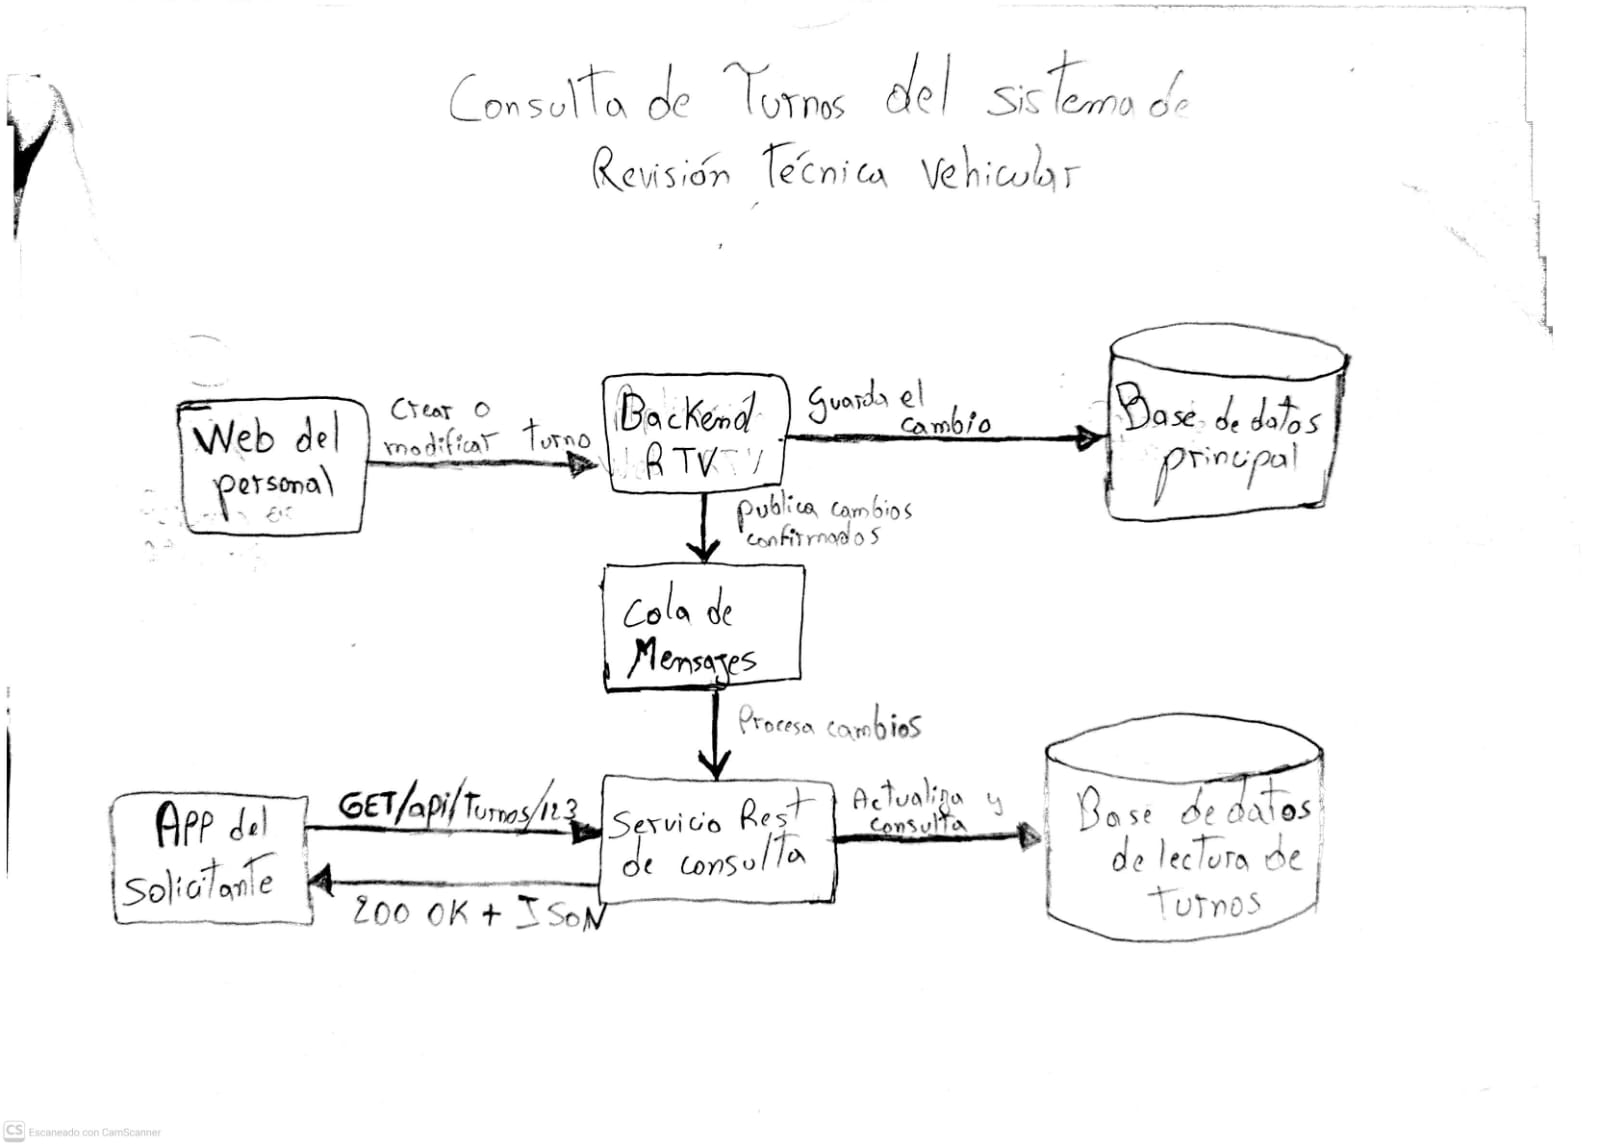
\includegraphics[width=\columnwidth,height=5.4cm,keepaspectratio]{../evidencias/kevin-bosquejo-rest-rtv.jpeg}

{\small Kevin García: consulta REST del RTV.}

\medskip
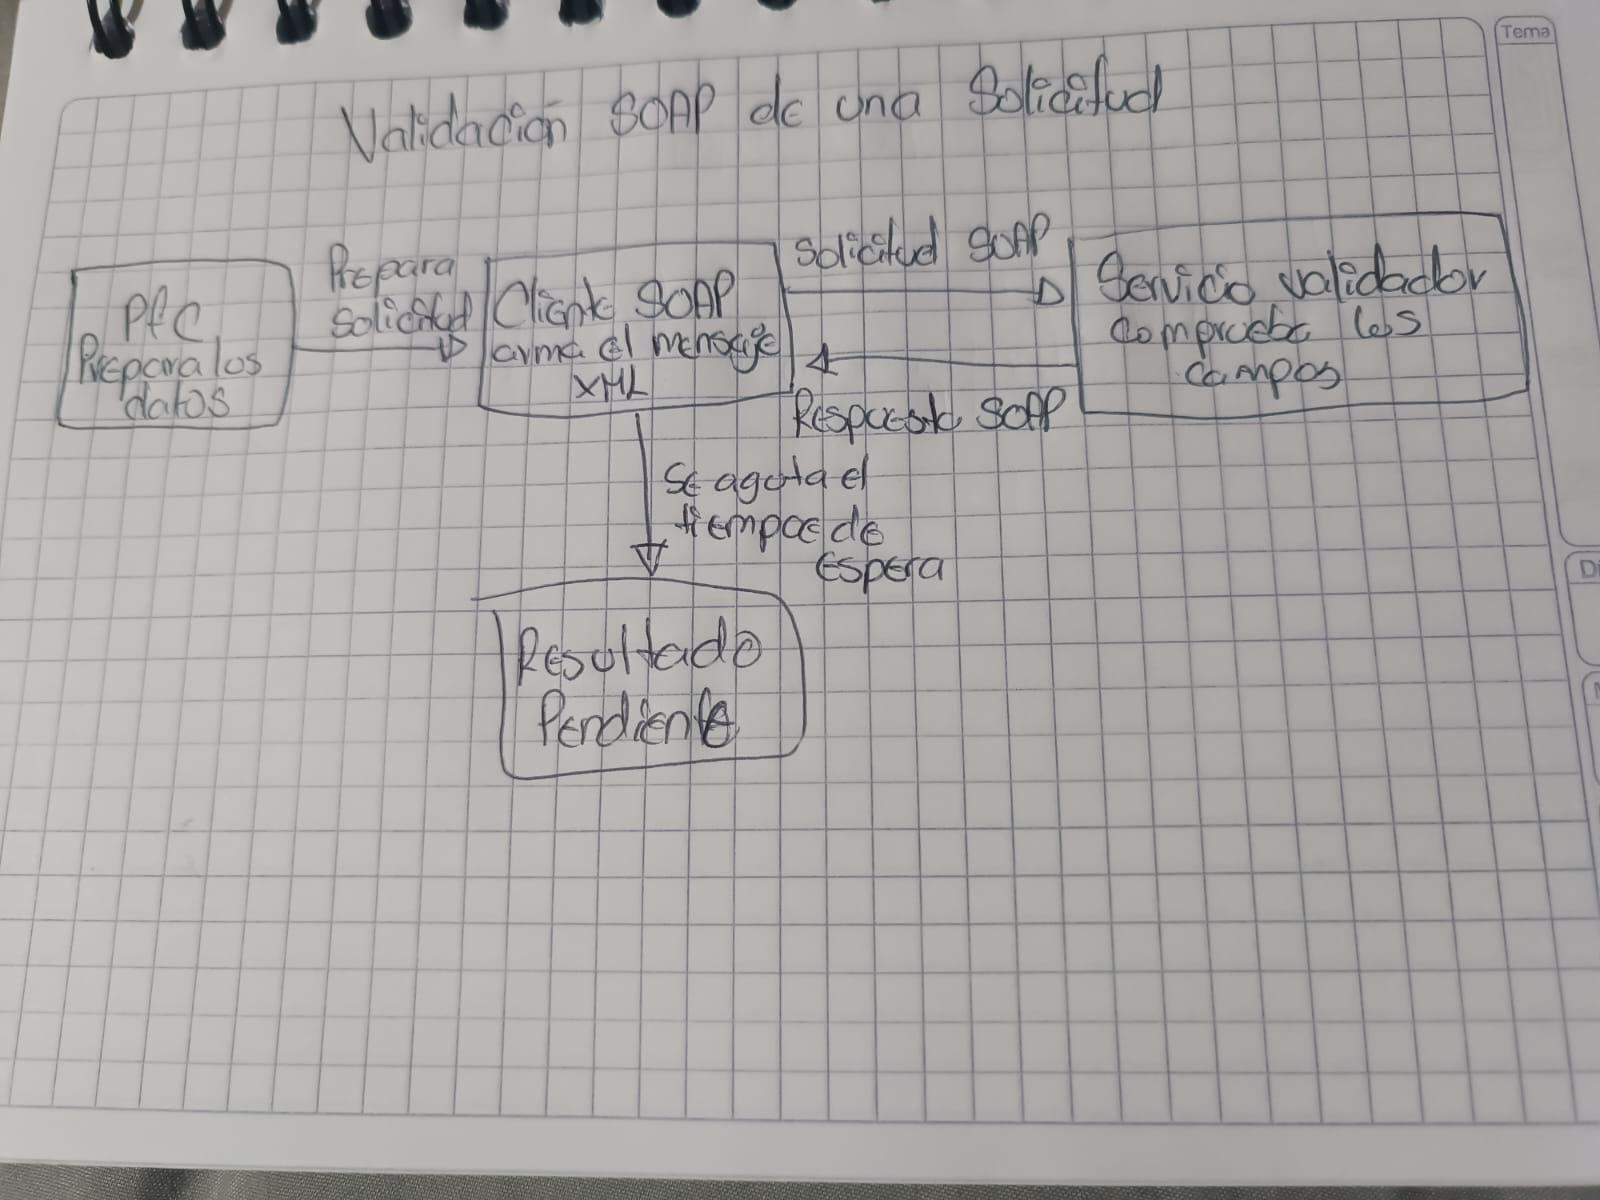
\includegraphics[width=\columnwidth,height=8.2cm,keepaspectratio]{../evidencias/juliana-bosquejo-soap.png}

{\small Juliana Emanuel: validación SOAP.}
\end{center}
\end{document}
